\section{Einleitung}
Hypothese:\\
Beispielhafte Ganganalyse für 7 Geschwindigkeiten.
Bewertung der Veränderung der Winkel und Trajektorien bei steigender Geschwindigkeit.

Identifikation wichtiger Schrittphasen anhand der Kräfte in Kopplung mit Trajektorien.\\

PLOT EINES GANGZYKLUSSES MIT KRÄFTEN DAZU!!\\
STICKPLOT?!?!\\
Nur Bezug auf Saggitalebene, hier Skizze rein mit beobachtete Gelenke


Die Analyse des menschlichen Ganges wird schon immer intensiv untersucht (Whittle1996). Die Anwendungsfelder reichen dabei  von der klinischen Forschung (Wren eta l 2011) über die Erforschung des Ganges in verschiedenen Situationen (QUELLE) bis hin zur Untersuchung von Laufmustern für Exoskelette oder Laufroboter (QUELLE). Die Evolution hat den zweibeinigen Gang dabei zu einem der energieffizientesten FOrtbwegeungsarten der Natur gemacht (QUELLE). Der sogenannte bipedale Gang fordert jedoch auch seinen Preis, da wir nicht immer einen stabilen Stand aufweisen. Um Energie zu sparen, verändern wir unseren Gang dabei mit der Geschwindigkeit deutlich.\\
hier Pendel, Eigenfrequenz verkürzen durch anwinkeln des Oberschenkels\\
Bewegt man sich mit der richtigen Geschwindigkeit fort, sodass die Pendelfrequenz der Eigenfrequenz eines Pendels der Beinlänge entspricht, benötigt die VOrwärtsbewegung des Beines am wenigsten Energie - das Laufen fühlt sich sehr angenehm an. Um solche Auswertungen durchzuführen wird der Gang am besten kinematisch untersucht. Zusätzlich zur Ganganalyse durch Bewegunsanalyse lassen sich auch über die Bodenreaktionskräfte (BRK) Aussagen über das Abfangen des Gewichtes sowie das Abstoßen machen. Abbildung EINS ABBILDUNG!! zeigt hier beispielsweise die verschiedenen Gangphasen sowie die auftretenden Bodenreaktionskräfte.
In dieser Arbeit wird exemplarisch der Gang eines Probanden kinematisch und kinetisch untersucht. Ziel dieser Arbeit ist es, den Einfluss verschiedener Gehgeschwindigkeiten beim gehen auf dem Laufband auf Schrittlänge und -frequenz zu untersuchen. Desweiteren wird das Gehen auf dem Laufband mit dem Gehen auf einer Laufstrecke verglichen. Auf letzterer werden zusätzlich die BRK aufgenommen. Dadurch können nicht nur die kinematischen Daten von Laufband und Laufstrecke untersucht werden, sondern zusätzlich die Bodenreaktionskräfte bei verschiedenen Geschwindigkeiten. Durhc Kombination der BRk und der Kinematik lässt sich durch inverse Kinematik die Kräfte und Momente in allen Gelenken ausrechnen und somit blablabla...

\begin{figure}
	\centering
	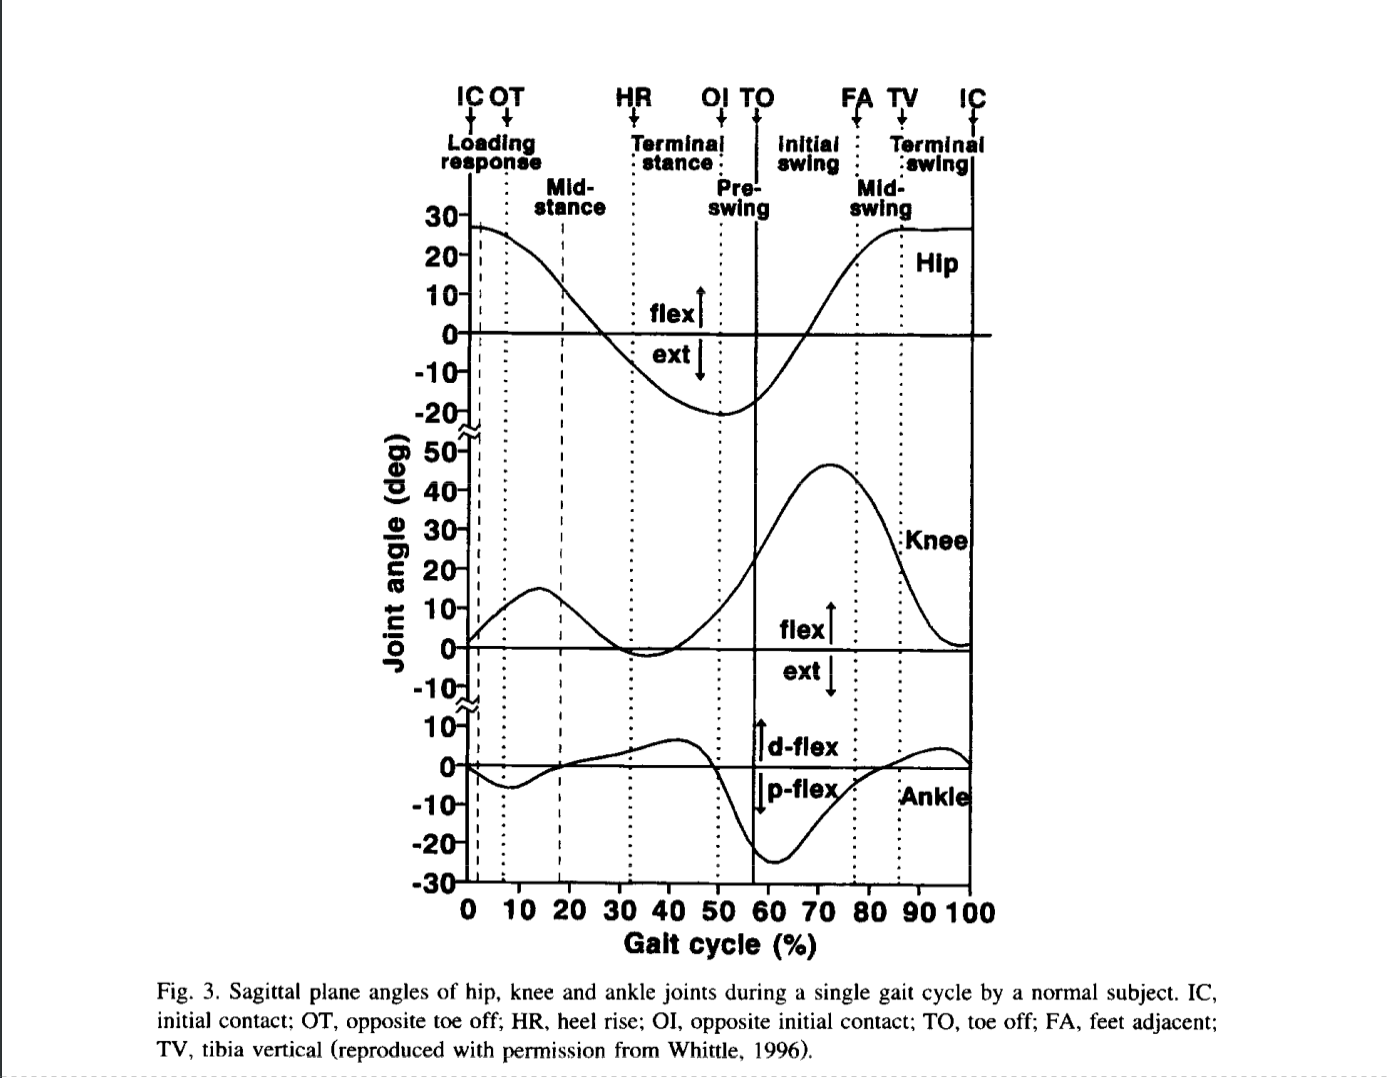
\includegraphics[width=0.7\linewidth]{bilder/Einleitung/gangphasen}
	\caption[Gangphasen]{blabla blabla}
	\label{fig:gangphasen}
\end{figure}


 Durch kinematische und kinetische Beobachtungen lassen sich diese 